
\documentclass[aspectratio=169]{beamer}

\usetheme{Madrid}
\usecolortheme{default}
\setbeamertemplate{navigation symbols}{}

\usepackage{graphicx}
\usepackage{booktabs}
\usepackage{amsmath, amssymb, mathtools}
\usepackage{pgfplots}
\usepackage{pgfplotstable}
\usepackage{hyperref}
\usepackage{tikz}
\usetikzlibrary{patterns,positioning,calc,matrix}
\pgfplotsset{compat=1.18}

% Allow compiling from either ./slides or project root.
\graphicspath{{../results/}{./results/}{./slides/}{./}}
\newcommand{\resultsdir}{../results/}
\IfFileExists{../results/german_credit_top_interactions.csv}{}{%
  \IfFileExists{./results/german_credit_top_interactions.csv}{\renewcommand{\resultsdir}{./results/}}{}%
}

\title[Purifying Interaction Effects]{Purifying Interaction Effects with Functional ANOVA:\\Paper Walkthrough + Two Experiments}
\author{Aik Tarkhanyan}
\date{}

% ---------- Convenience macros ----------
\newcommand{\wemp}{\hat w_{\mathrm{emp}}}
\newcommand{\wunif}{\hat w_{\mathrm{unif}}}
\newcommand{\wlap}{\hat w_{\mathrm{lap}}}
\newcommand{\windep}{w_{\mathrm{indep}}}
\newcommand{\wperm}{w_{\mathrm{perm}}}
\newcommand{\rhoVal}{\rho}

\newcommand{\Ew}{\mathbb{E}_{w}}
\newcommand{\Varw}{\mathrm{Var}_{w}}

% ---------- Small callout boxes ----------
\newcommand{\TakeawayBox}[1]{%
  \vspace{0.25em}%
  {\footnotesize
  \begin{beamercolorbox}[rounded=true,sep=0.6ex,wd=\linewidth]{block body}
    \textbf{Takeaway:} #1%
  \end{beamercolorbox}}%
}

% ---------- Agenda slide command with optional highlighting ----------
\newcommand{\AgendaSlide}[1][0]{%
\begin{frame}{Agenda}
\small
\begin{columns}[T]
\begin{column}{0.48\textwidth}
\textbf{Part I: Paper Walkthrough}
\begin{enumerate}
  \item[\ifnum#1=1\color{blue!80}$\blacktriangleright$\else\fi 1.] \ifnum#1=1\textbf{\color{blue!80}The identifiability problem}\else The identifiability problem\fi
  \item[\ifnum#1=2\color{blue!80}$\blacktriangleright$\else\fi 2.] \ifnum#1=2\textbf{\color{blue!80}Functional ANOVA target}\else Functional ANOVA target\fi
  \item[\ifnum#1=3\color{blue!80}$\blacktriangleright$\else\fi 3.] \ifnum#1=3\textbf{\color{blue!80}Mass-moving algorithm}\else Mass-moving algorithm\fi
  \item[\ifnum#1=4\color{blue!80}$\blacktriangleright$\else\fi 4.] \ifnum#1=4\textbf{\color{blue!80}Convergence \& properties}\else Convergence \& properties\fi
  \item[\ifnum#1=5\color{blue!80}$\blacktriangleright$\else\fi 5.] \ifnum#1=5\textbf{\color{blue!80}Weight estimation ($w$)}\else Weight estimation ($w$)\fi
\end{enumerate}
\end{column}
\begin{column}{0.48\textwidth}
\textbf{Part II: Experiments}
\begin{enumerate}
  \item[\ifnum#1=6\color{blue!80}$\blacktriangleright$\else\fi 6.] \ifnum#1=6\textbf{\color{blue!80}German Credit (real data)}\else German Credit (real data)\fi\\
    {\scriptsize Main effects \& interactions under different $w$}
  \item[\ifnum#1=7\color{blue!80}$\blacktriangleright$\else\fi 7.] \ifnum#1=7\textbf{\color{blue!80}Stress-test (synthetic)}\else Stress-test (synthetic)\fi\\
    {\scriptsize How dependence $\rho$ affects purification}
\end{enumerate}
\vspace{1em}
\textbf{Conclusions}
\begin{itemize}
  \item[\ifnum#1=8\color{blue!80}$\blacktriangleright$\else\fi] \ifnum#1=8\textbf{\color{blue!80}Summary \& takeaways}\else Summary \& takeaways\fi
\end{itemize}
\end{column}
\end{columns}
\end{frame}
}

% ---------- Section divider: show agenda with current section highlighted ----------
\AtBeginSection[]{%
  \ifnum\insertsectionnumber=1\relax
    \AgendaSlide[1]
  \else\ifnum\insertsectionnumber=2\relax
    \AgendaSlide[6]
  \else\ifnum\insertsectionnumber=3\relax
    \AgendaSlide[7]
  \fi\fi\fi
}

\begin{document}

% ============================================================
\begin{frame}
  \titlepage
  \vspace{-1em}
  \centering
  {\footnotesize \url{https://github.com/HaykTarkhanyan/fanova_purification}}
\end{frame}

% ============================================================
\AgendaSlide[0]

% ============================================================
\section{Paper walkthrough}

% ============================================================
\begin{frame}{1) Additive models with interactions}
\small
	We consider models of the form:
\[
Y \approx f_0 + f_1(X_1) + f_2(X_2) + f_3(X_1,X_2)
\]
More generally:
\[
F(X) = f_0 + \sum_{i=1}^d f_i(X_i) + \sum_{i\neq j} f_{ij}(X_i,X_j) + \cdots
\]
\begin{itemize}
  \item Goal: interpret $f_i$ (mains) and $f_{ij}$ (interactions).
  \item Problem: without constraints, the decomposition is \textbf{non-identifiable}.
\end{itemize}
\end{frame}

% ============================================================
\begin{frame}{2) Identifiability issue: effects can move across orders}
\small
For a fixed predictor, you can shift ``mass'' between terms while keeping predictions identical.

\vspace{0.5em}
\begin{block}{Simple intuition}
Add any $h(X_1)$ to $f_1$ and subtract the same $h(X_1)$ from $f_{12}(X_1,X_2)$: the sum stays unchanged.
\end{block}

\vspace{0.5em}
\begin{itemize}
  \item This allows \textbf{contradictory interpretations} for the exact same function.
  \item So ``main effect'' and ``interaction'' are not uniquely defined by the predictor.
  \item This motivates a \textbf{canonical} notion of ``pure'' interactions.
\end{itemize}
\end{frame}

% ============================================================
	\begin{frame}{3) Boolean example (OR/AND as XOR + mains)}
\small
Let $X_1,X_2\in\{0,1\}$.

\vspace{0.4em}
	\begin{block}{Key equivalence}
\[
X_1 \vee X_2 
= 0.25\,(X_1 \oplus X_2)
+ 0.5\,(X_1-0.5)
+ 0.5\,(X_2-0.5)
+ 0.75
\]
\end{block}

\vspace{0.4em}
Similarly:
\[
X_1 \wedge X_2 
= -0.25\,(X_1 \oplus X_2)
+ 0.5\,(X_1-0.5)
+ 0.5\,(X_2-0.5)
+ 0.25
\]

\begin{itemize}
  \item The interaction parts are (centered) XOR up to sign; the rest is absorbed into mains+intercept.
  \item AND and OR have identical interaction structure (centered XOR up to sign); differences are absorbed into mains/intercept.
\end{itemize}
\end{frame}

% ============================================================
\begin{frame}{Representational degeneracy}
\centering
\includegraphics[width=0.98\linewidth,height=0.74\textheight,keepaspectratio]{figures_manual/different_interactions_same_output.png}
\TakeawayBox{Multiple decompositions can yield identical predictions but assign credit differently across mains/interactions; purification selects a canonical one.}
\end{frame}

% ============================================================
\begin{frame}{4) Multiplicative model and the $(\alpha,\beta)$ degree of freedom}
\small
A classic interaction model:
\[
Y \approx a + bX_1 + cX_2 + dX_1X_2.
\]
		An equivalent re-parameterization (for any $\alpha,\beta$):
\[
Y \approx (a - d\alpha\beta) + (b + d\beta)X_1 + (c + d\alpha)X_2 + d\,(X_1-\alpha)(X_2-\beta).
\]
\begin{itemize}
  \item Identifiable as a function, but coefficients are \textbf{not meaningful} without rules for choosing $\alpha,\beta$.
		  \item A canonical choice is the fANOVA one, which yields \textbf{minimum variance in higher-order terms}.
  \item Conceptually, centering constants align with moments like $\Ew[X_1]$ and $\Ew[X_2]$; the decomposition depends on $w$.
\end{itemize}
\end{frame}

% ============================================================
\begin{frame}{Multiplicative example: varying $(\alpha,\beta)$}
\centering
\includegraphics[width=0.93\linewidth,height=0.73\textheight,keepaspectratio]{figures_manual/multiplicative_example_varying_alpha_beta.png}
\TakeawayBox{As $(\alpha,\beta)$ vary, variance attribution shifts between mains and interactions even though predictions do not.}
\end{frame}

% ============================================================
\begin{frame}{5) Functional ANOVA (fANOVA): the canonical target}
\small
The functional ANOVA decomposes $F$ into \textbf{orthogonal} components under weight $w(X)$:
\[
\underbrace{F(X)}_{\text{predictor}} = \underbrace{f_0}_{\text{intercept}} + \underbrace{\sum_{i} f_i(X_i)}_{\text{main effects}} + \underbrace{\sum_{i<j} f_{ij}(X_i,X_j)}_{\text{pairwise interactions}} + \cdots
\]

\vspace{0.3em}
\textbf{Orthogonality:} $\;\Ew[f_u \cdot f_v] = 0$ for $u \neq v$.

\vspace{0.3em}
Equivalently, each component satisfies \textbf{integrate-to-zero} (marginalizing out any variable gives 0):
\[
\boxed{\Ew[f_u(X_u) \mid X_{u \setminus i}] = 0 \quad \forall\, i \in u}
\]
\vspace{-0.3em}
\begin{itemize}
  \item For main effect $f_i$: $\;\Ew[f_i(X_i)] = 0$ (centered).
  \item For interaction $f_{ij}$: $\;\Ew[f_{ij} \mid X_i] = 0$ and $\Ew[f_{ij} \mid X_j] = 0$ (no marginal structure).
\end{itemize}
\end{frame}

% ============================================================
\begin{frame}{6) Piecewise-constant case: tensors + slice mean-zero}
\small
For piecewise-constant $F$ on bins (one set per feature), each $f_u$ becomes a \textbf{tensor} $T_u$.

\vspace{0.3em}
\textbf{Integrate-to-zero} $\to$ \textbf{weighted slice mean-zero}:
\[
\boxed{\sum_{k} T_u[\ldots, k, \ldots] \cdot w_i[k] = 0 \quad \text{for each slice along dimension } i \in u}
\]

\vspace{0.3em}
\begin{block}{Pairwise intuition ($f_{ij}$ is a matrix)}
\begin{itemize}
  \item Each \textbf{row} has weighted mean zero: $\sum_k T_{ij}[r, k] \cdot w_j[k] = 0$
  \item Each \textbf{column} has weighted mean zero: $\sum_k T_{ij}[k, c] \cdot w_i[k] = 0$
\end{itemize}
\end{block}

\TakeawayBox{This constraint enables an exact post-hoc algorithm for tree ensembles.}
\end{frame}

% ============================================================
\begin{frame}{Slice Mean-Zero: Visual Example}
\begin{columns}[c]
  \begin{column}{0.48\textwidth}
    \centering
    \textbf{Before purification}\\[0.5em]
    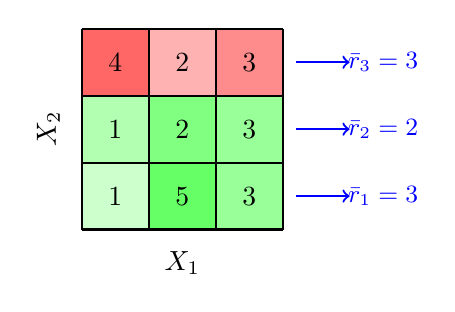
\begin{tikzpicture}[scale=0.85]
      % Grid
      \fill[red!60] (0,2) rectangle (1,3);
      \fill[red!30] (1,2) rectangle (2,3);
      \fill[red!45] (2,2) rectangle (3,3);
      \fill[green!30] (0,1) rectangle (1,2);
      \fill[green!50] (1,1) rectangle (2,2);
      \fill[green!40] (2,1) rectangle (3,2);
      \fill[green!20] (0,0) rectangle (1,1);
      \fill[green!60] (1,0) rectangle (2,1);
      \fill[green!40] (2,0) rectangle (3,1);
      \draw[thick] (0,0) grid (3,3);
      % Values
      \node at (0.5,2.5) {4};
      \node at (1.5,2.5) {2};
      \node at (2.5,2.5) {3};
      \node at (0.5,1.5) {1};
      \node at (1.5,1.5) {2};
      \node at (2.5,1.5) {3};
      \node at (0.5,0.5) {1};
      \node at (1.5,0.5) {5};
      \node at (2.5,0.5) {3};
      % Row means
      \draw[->,thick,blue] (3.2,2.5) -- (4.0,2.5);
      \node[blue,font=\small] at (4.5,2.5) {$\bar{r}_3=3$};
      \draw[->,thick,blue] (3.2,1.5) -- (4.0,1.5);
      \node[blue,font=\small] at (4.5,1.5) {$\bar{r}_2=2$};
      \draw[->,thick,blue] (3.2,0.5) -- (4.0,0.5);
      \node[blue,font=\small] at (4.5,0.5) {$\bar{r}_1=3$};
      % Labels
      \node[rotate=90] at (-0.5,1.5) {$X_2$};
      \node at (1.5,-0.5) {$X_1$};
    \end{tikzpicture}
    
    \vspace{0.5em}
    {\small Row means $\neq 0$}
  \end{column}
  
  \begin{column}{0.48\textwidth}
    \centering
    \textbf{After purification}\\[0.5em]
    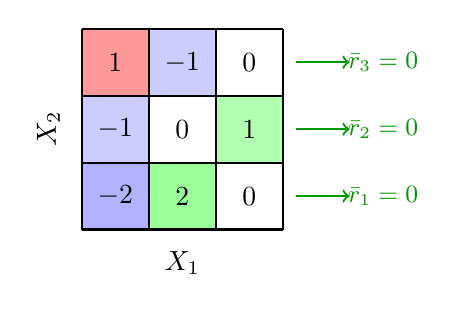
\begin{tikzpicture}[scale=0.85]
      % Grid - purified (row means = 0)
      \fill[red!40] (0,2) rectangle (1,3);
      \fill[blue!20] (1,2) rectangle (2,3);
      \fill[white] (2,2) rectangle (3,3);
      \fill[blue!20] (0,1) rectangle (1,2);
      \fill[white] (1,1) rectangle (2,2);
      \fill[green!30] (2,1) rectangle (3,2);
      \fill[blue!30] (0,0) rectangle (1,1);
      \fill[green!40] (1,0) rectangle (2,1);
      \fill[white] (2,0) rectangle (3,1);
      \draw[thick] (0,0) grid (3,3);
      % Values (centered)
      \node at (0.5,2.5) {1};
      \node at (1.5,2.5) {$-$1};
      \node at (2.5,2.5) {0};
      \node at (0.5,1.5) {$-$1};
      \node at (1.5,1.5) {0};
      \node at (2.5,1.5) {1};
      \node at (0.5,0.5) {$-$2};
      \node at (1.5,0.5) {2};
      \node at (2.5,0.5) {0};
      % Row means = 0
      \draw[->,thick,green!60!black] (3.2,2.5) -- (4.0,2.5);
      \node[green!60!black,font=\small] at (4.5,2.5) {$\bar{r}_3=0$};
      \draw[->,thick,green!60!black] (3.2,1.5) -- (4.0,1.5);
      \node[green!60!black,font=\small] at (4.5,1.5) {$\bar{r}_2=0$};
      \draw[->,thick,green!60!black] (3.2,0.5) -- (4.0,0.5);
      \node[green!60!black,font=\small] at (4.5,0.5) {$\bar{r}_1=0$};
      % Labels
      \node[rotate=90] at (-0.5,1.5) {$X_2$};
      \node at (1.5,-0.5) {$X_1$};
    \end{tikzpicture}
    
    \vspace{0.5em}
    {\small Row means $= 0$ {\color{green!60!black}\checkmark}}
  \end{column}
\end{columns}

\vspace{0.8em}
\begin{block}{What happens to the removed mass?}
Row means are subtracted from the interaction tensor $\to$ added to the main effect $f_2(X_2)$.\\
Column means are subtracted $\to$ added to $f_1(X_1)$. Predictions unchanged!
\end{block}
\end{frame}

% ============================================================
\begin{frame}{7) ``Pure interaction effects'' = fANOVA of $\mathbb{E}[Y\mid X]$}
\small
\textbf{Pure interactions} = variance that \emph{cannot} be explained by any subset of variables.

\vspace{0.4em}
\begin{block}{Formal definition}
Find $\{f_u\}$ that minimize $\Ew\bigl[(F(X) - \sum_u f_u(X_u))^2\bigr]$ subject to:
\[
\Ew[f_u(X_u) \mid X_v] = 0 \quad \forall\, v \subsetneq u
\]
\end{block}

\vspace{0.3em}
\begin{alertblock}{Key insight}
This is exactly the fANOVA decomposition with $w(X) = p(X)$ (true data density).
\end{alertblock}

\TakeawayBox{Pure = irreducible. If $f_{ij}$ can be absorbed into $f_i$ or $f_j$, it's not a ``pure'' interaction.}
\end{frame}

% ============================================================
\begin{frame}{8) Purification for trees: mass-moving}
\small
For tree ensembles, represent effects as tensors $T_u$. \textbf{Idea}: iteratively move weighted slice means from higher-order to lower-order tensors.

\vspace{0.4em}
\begin{block}{One step of mass-moving}
\begin{enumerate}
  \item Compute weighted mean of slice: $\bar{m} = \sum_k T_u[\ldots,k,\ldots] \cdot w_i[k]$
  \item Subtract from interaction: $T_u[\ldots,k,\ldots] \;\leftarrow\; T_u[\ldots,k,\ldots] - \bar{m}$
  \item Add to lower-order tensor: $T_{u\setminus i}[\ldots] \;\leftarrow\; T_{u\setminus i}[\ldots] + \bar{m}$
\end{enumerate}
\end{block}

\vspace{0.3em}
\textbf{Algorithm}:
\begin{itemize}
  \item \textbf{Purify-Matrix}: cycle through dimensions until all slice means $\approx 0$.
  \item \textbf{Purify-All}: process tensors from highest-order down to intercept.
\end{itemize}
\end{frame}



% ============================================================
\begin{frame}{Mass-moving (Purify-Matrix): Visual Walkthrough}
\small
\begin{center}
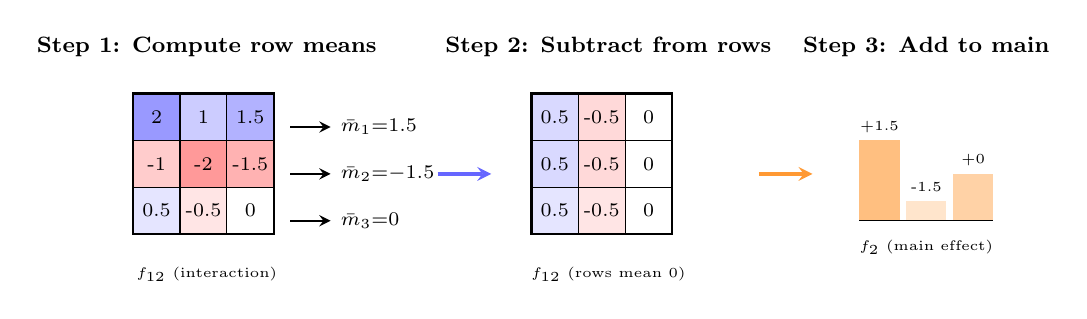
\begin{tikzpicture}[scale=0.85,
  box/.style={draw,minimum width=0.7cm,minimum height=0.7cm,font=\scriptsize},
  arr/.style={->,thick,>=stealth}]
  
  % Step 1: Interaction tensor with non-zero row means
  \node[font=\footnotesize\bfseries] at (1.05,3.2) {Step 1: Compute row means};
  % Manual 3x3 grid instead of matrix
  \begin{scope}[shift={(-0.05,0.4)}]
    % Row 1
    \fill[blue!40] (0,1.4) rectangle (0.7,2.1); \node[font=\scriptsize] at (0.35,1.75) {2};
    \fill[blue!20] (0.7,1.4) rectangle (1.4,2.1); \node[font=\scriptsize] at (1.05,1.75) {1};
    \fill[blue!30] (1.4,1.4) rectangle (2.1,2.1); \node[font=\scriptsize] at (1.75,1.75) {1.5};
    % Row 2
    \fill[red!20] (0,0.7) rectangle (0.7,1.4); \node[font=\scriptsize] at (0.35,1.05) {-1};
    \fill[red!40] (0.7,0.7) rectangle (1.4,1.4); \node[font=\scriptsize] at (1.05,1.05) {-2};
    \fill[red!30] (1.4,0.7) rectangle (2.1,1.4); \node[font=\scriptsize] at (1.75,1.05) {-1.5};
    % Row 3
    \fill[blue!10] (0,0) rectangle (0.7,0.7); \node[font=\scriptsize] at (0.35,0.35) {0.5};
    \fill[red!10] (0.7,0) rectangle (1.4,0.7); \node[font=\scriptsize] at (1.05,0.35) {-0.5};
    \fill[white] (1.4,0) rectangle (2.1,0.7); \draw (1.4,0) rectangle (2.1,0.7); \node[font=\scriptsize] at (1.75,0.35) {0};
    \draw[thick] (0,0) rectangle (2.1,2.1);
    \draw (0,0.7) -- (2.1,0.7); \draw (0,1.4) -- (2.1,1.4);
    \draw (0.7,0) -- (0.7,2.1); \draw (1.4,0) -- (1.4,2.1);
  \end{scope}
  \node[font=\tiny] at (1.05,-0.2) {$f_{12}$ (interaction)};
  % Row means on right
  \draw[arr] (2.3,2.0) -- (2.9,2.0) node[right,font=\scriptsize] {$\bar{m}_1{=}1.5$};
  \draw[arr] (2.3,1.3) -- (2.9,1.3) node[right,font=\scriptsize] {$\bar{m}_2{=}{-}1.5$};
  \draw[arr] (2.3,0.6) -- (2.9,0.6) node[right,font=\scriptsize] {$\bar{m}_3{=}0$};
  
  % Arrow to step 2
  \draw[arr,very thick,blue!60] (4.5,1.3) -- (5.3,1.3);
  
  % Step 2: Subtract means from rows
  \node[font=\footnotesize\bfseries] at (7.05,3.2) {Step 2: Subtract from rows};
  \begin{scope}[shift={(5.9,0.4)}]
    % All rows now have values centered around 0
    \fill[blue!15] (0,1.4) rectangle (0.7,2.1); \node[font=\scriptsize] at (0.35,1.75) {0.5};
    \fill[red!15] (0.7,1.4) rectangle (1.4,2.1); \node[font=\scriptsize] at (1.05,1.75) {-0.5};
    \fill[white] (1.4,1.4) rectangle (2.1,2.1); \draw (1.4,1.4) rectangle (2.1,2.1); \node[font=\scriptsize] at (1.75,1.75) {0};
    \fill[blue!15] (0,0.7) rectangle (0.7,1.4); \node[font=\scriptsize] at (0.35,1.05) {0.5};
    \fill[red!15] (0.7,0.7) rectangle (1.4,1.4); \node[font=\scriptsize] at (1.05,1.05) {-0.5};
    \fill[white] (1.4,0.7) rectangle (2.1,1.4); \draw (1.4,0.7) rectangle (2.1,1.4); \node[font=\scriptsize] at (1.75,1.05) {0};
    \fill[blue!10] (0,0) rectangle (0.7,0.7); \node[font=\scriptsize] at (0.35,0.35) {0.5};
    \fill[red!10] (0.7,0) rectangle (1.4,0.7); \node[font=\scriptsize] at (1.05,0.35) {-0.5};
    \fill[white] (1.4,0) rectangle (2.1,0.7); \draw (1.4,0) rectangle (2.1,0.7); \node[font=\scriptsize] at (1.75,0.35) {0};
    \draw[thick] (0,0) rectangle (2.1,2.1);
    \draw (0,0.7) -- (2.1,0.7); \draw (0,1.4) -- (2.1,1.4);
    \draw (0.7,0) -- (0.7,2.1); \draw (1.4,0) -- (1.4,2.1);
  \end{scope}
  \node[font=\tiny] at (7.05,-0.2) {$f_{12}$ (rows mean 0)};
  
  % Arrow to step 3
  \draw[arr,very thick,orange!80] (9.3,1.3) -- (10.1,1.3);
  
  % Step 3: Add to main effect
  \node[font=\footnotesize\bfseries] at (11.8,3.2) {Step 3: Add to main};
  \begin{scope}[shift={(10.8,0.6)}]
    \fill[orange!50] (0,0) rectangle (0.6,1.2);
    \fill[orange!20] (0.7,0) rectangle (1.3,0.3);
    \fill[orange!35] (1.4,0) rectangle (2.0,0.7);
    \draw (0,0) -- (2.0,0);
    \node[font=\tiny] at (1.0,-0.4) {$f_2$ (main effect)};
    \node[font=\tiny] at (0.3,1.4) {+1.5};
    \node[font=\tiny] at (1.0,0.5) {-1.5};
    \node[font=\tiny] at (1.7,0.9) {+0};
  \end{scope}
\end{tikzpicture}
\end{center}

\vspace{-0.3em}
\begin{columns}[T]
  \begin{column}{0.55\textwidth}
    \begin{block}{\small Key insight}
    \scriptsize
    Subtracting $\bar{m}_i$ from row $i$ of $f_{12}$ and adding it to $f_2[i]$ preserves predictions:
    \[
    f_2(x_2) + f_{12}(x_1,x_2) = \text{unchanged}
    \]
    \end{block}
  \end{column}
  \begin{column}{0.43\textwidth}
    \begin{block}{\small Result}
    \scriptsize
    After convergence: every row/column of interaction has weighted mean = 0
    \end{block}
  \end{column}
\end{columns}

\TakeawayBox{Mass moves from interaction to mains; predictions stay identical; interaction becomes ``pure'' (only irreducible structure remains).}
\end{frame}



\begin{frame}{Example: COMPAS + Recidivism Datasets}
\centering
\includegraphics[width=0.98\linewidth,height=0.78\textheight,keepaspectratio]{figures_manual/compas_example.png}
\end{frame}

% ============================================================
\begin{frame}{COMPAS Dataset}
\begin{columns}[T]
\begin{column}{0.5\textwidth}
\centering
\includegraphics[width=\linewidth,height=0.78\textheight,keepaspectratio]{figures_manual/compass.png}
\end{column}
\begin{column}{0.48\textwidth}
\footnotesize
\textbf{What is COMPAS?}
\begin{itemize}\setlength{\itemsep}{2pt}
  \item Predicts recidivism risk for bail decisions
  \item High stakes $\rightarrow$ fair treatment crucial
\end{itemize}

\vspace{0.3em}
\textbf{Key Insights:}
\begin{itemize}\setlength{\itemsep}{2pt}
  \item Main effects \textbf{change significantly} after purification
  \item Magnitude and \textbf{sign} depend on weight choice
  \item XGB signs often \textbf{opposite} to purified models
\end{itemize}
\end{column}
\end{columns}
\end{frame}

% ============================================================
\begin{frame}{Recidivism Dataset}
\begin{columns}[T]
\begin{column}{0.5\textwidth}
\centering
\includegraphics[width=\linewidth,height=0.78\textheight,keepaspectratio]{figures_manual/recidivism.png}
\end{column}
\begin{column}{0.48\textwidth}
\footnotesize
\textbf{Background:}
\begin{itemize}\setlength{\itemsep}{2pt}
  \item Propublica 2016: Broward County, FL
  \item Includes COMPAS predictions
\end{itemize}

\vspace{0.3em}
\textbf{Why It Matters:}
\begin{itemize}\setlength{\itemsep}{2pt}
  \item Sparked algorithmic bias controversy
  \item Conflicting conclusions across studies
\end{itemize}

\vspace{0.3em}
\textbf{Research Question:}\\[2pt]
Does purification change bias conclusions?
\end{column}
\end{columns}
\end{frame}

% ============================================================
\begin{frame}{Example: California housing}
\centering
\includegraphics[width=0.98\linewidth,height=0.78\textheight,keepaspectratio]{figures_manual/california_example.png}
\end{frame}

% ============================================================
\begin{frame}{10) Convergence + correctness}
\small
The mass-moving procedure converges to tensors satisfying slice mean-zero constraints.
In practice, a small number of sweeps per interaction tensor is enough (see next slide).

\vspace{0.5em}
\begin{block}{Theorem 1 (special distributions)}
For many simple weights (e.g., uniform along row/column dimensions), purification converges in a single pass.
\end{block}

\vspace{0.4em}
	\begin{block}{Theorem 2 (generic non-degenerate $w$)}
	Converges to tolerance $\varepsilon$ in $O(\log(M_0)-\log(\varepsilon))$ iterations per interaction tensor.\\[3pt]
	{\footnotesize $M_0$ = initial unpurified mass $\sum_{i,j} w_{i,j}(r_i + c_j)$, where $r_i, c_j$ are row/column means.}
	\end{block}
	\end{frame}

	% ============================================================
\begin{frame}{Empirical convergence: mass moves quickly}
\small
\begin{columns}[T,onlytextwidth]
  \begin{column}{0.46\linewidth}
    \begin{itemize}
      \item Generate random tensors $T \sim \mathcal{N}(0,\sigma I)$.
      \item Use weights either:
            (i) uniform ($w \propto 1$) or
            (ii) Gaussian ($w \sim \mathcal{N}(0,\sigma I)$) in dimension $P$.
      \item In practice, almost all mass is moved in the first iteration.
      \item With uniform weights, convergence occurs in a single pass (per row/column).
    \end{itemize}
    \TakeawayBox{Most of the mass moves on the first sweep; uniform weights converge in one pass, enabling purification at scale.}
  \end{column}
  \begin{column}{0.54\linewidth}
    \centering
		\includegraphics[width=\linewidth]{figures_manual/mass_quickly_moved.png}
  \end{column}
\end{columns}
\end{frame}
	
	% ============================================================
\begin{frame}{11) Useful properties}
\small
Because the purified decomposition is the unique fANOVA form:
\begin{itemize}
  \item \textbf{Permutation invariance:} reordering categorical codes does not change purified interactions.
  \item \textbf{Linearity:} purification commutes with averaging / bagging (purify ensembles without changing results).
\end{itemize}
\end{frame}

% ============================================================
		\begin{frame}{12) Estimating $w$ is part of interpretation}
	\small
		Effects are only meaningful \emph{relative to} a distribution $w(X)$.
	The correct target is the true data density $p(X)$, but it must be estimated.

\vspace{0.5em}
\begin{block}{Three practical estimators (piecewise-constant)}
\begin{itemize}
  \item \textbf{Uniform:} $\wunif(x_{-u}) \propto 1$
  \item \textbf{Empirical:} $\wemp(x_{-u}) \propto \sum_{x\in X_{\mathrm{train}}} \mathbf{1}\{x_{-u}=x_{-u}'\}$
  \item \textbf{Laplace:} $\wlap \propto \wunif + \wemp$ (avoids zero-count bins; stabilizes slice means when support is sparse)
\end{itemize}
	\end{block}
	\end{frame}

% ============================================================
\begin{frame}{Binning \& Weight Distributions}
\begin{columns}[T]
  \begin{column}{0.55\textwidth}
    \centering
    \textbf{Tree splits $\to$ bins}\\[0.5em]
    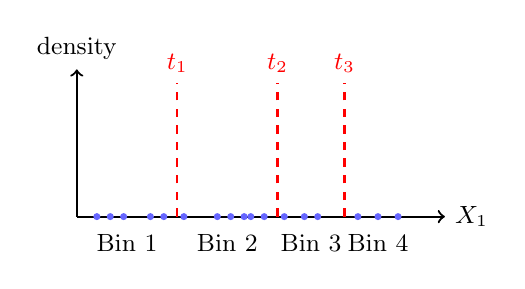
\begin{tikzpicture}[scale=0.85]
      % Axis
      \draw[->,thick] (0,0) -- (5.5,0) node[right,font=\small] {$X_1$};
      \draw[->,thick] (0,0) -- (0,2.2) node[above,font=\small] {density};
      
      % Data points (scattered)
      \foreach \x in {0.3,0.5,0.7,1.1,1.3,1.6,2.1,2.3,2.5,2.6,2.8,3.1,3.4,3.6,4.2,4.5,4.8} {
        \fill[blue!60] (\x,0) circle (1.5pt);
      }
      
      % Split thresholds
      \draw[red,thick,dashed] (1.5,0) -- (1.5,2.0) node[above,font=\small] {$t_1$};
      \draw[red,thick,dashed] (3.0,0) -- (3.0,2.0) node[above,font=\small] {$t_2$};
      \draw[red,thick,dashed] (4.0,0) -- (4.0,2.0) node[above,font=\small] {$t_3$};
      
      % Bin labels
      \node[font=\small] at (0.75,-0.4) {Bin 1};
      \node[font=\small] at (2.25,-0.4) {Bin 2};
      \node[font=\small] at (3.5,-0.4) {Bin 3};
      \node[font=\small] at (4.5,-0.4) {Bin 4};
    \end{tikzpicture}
  \end{column}
  
  \begin{column}{0.42\textwidth}
    \begin{block}{Weight options}
    \small
    \begin{tabular}{@{}ll@{}}
      \textbf{uniform} & All bins equal \\[0.3em]
      \textbf{empirical} & Counts from data \\[0.3em]
      \textbf{laplace} & empirical + smooth \\[0.3em]
      \textbf{indep} & $w_{12} {=} w_1 {\cdot} w_2$
    \end{tabular}
    \end{block}
  \end{column}
\end{columns}

\vspace{0.8em}
\begin{columns}[T]
  \begin{column}{0.48\textwidth}
    \centering
    \textbf{Uniform weights}\\[0.3em]
    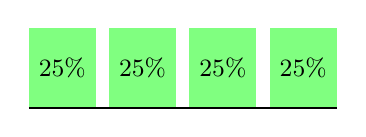
\begin{tikzpicture}[scale=0.85]
      \fill[green!50] (0,0) rectangle (1,1.2);
      \fill[green!50] (1.2,0) rectangle (2.2,1.2);
      \fill[green!50] (2.4,0) rectangle (3.4,1.2);
      \fill[green!50] (3.6,0) rectangle (4.6,1.2);
      \draw[thick] (0,0) -- (4.6,0);
      \node[font=\small] at (0.5,0.6) {25\%};
      \node[font=\small] at (1.7,0.6) {25\%};
      \node[font=\small] at (2.9,0.6) {25\%};
      \node[font=\small] at (4.1,0.6) {25\%};
    \end{tikzpicture}
  \end{column}
  
  \begin{column}{0.48\textwidth}
    \centering
    \textbf{Empirical weights}\\[0.3em]
    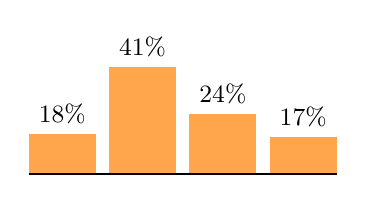
\begin{tikzpicture}[scale=0.85]
      \fill[orange!70] (0,0) rectangle (1,0.6);
      \fill[orange!70] (1.2,0) rectangle (2.2,1.6);
      \fill[orange!70] (2.4,0) rectangle (3.4,0.9);
      \fill[orange!70] (3.6,0) rectangle (4.6,0.55);
      \draw[thick] (0,0) -- (4.6,0);
      \node[font=\small,above] at (0.5,0.6) {18\%};
      \node[font=\small,above] at (1.7,1.6) {41\%};
      \node[font=\small,above] at (2.9,0.9) {24\%};
      \node[font=\small,above] at (4.1,0.55) {17\%};
    \end{tikzpicture}
  \end{column}
\end{columns}

\vspace{0.5em}
\TakeawayBox{Bins derived from tree splits. Weight choice affects the ``slice mean zero'' constraint.}
\end{frame}

% ============================================================
\begin{frame}{2D Joint Weights: Correlated Features}
\begin{columns}[c]
  \begin{column}{0.48\textwidth}
    \centering
    \textbf{$\wemp$ (true joint)}\\[0.4em]
    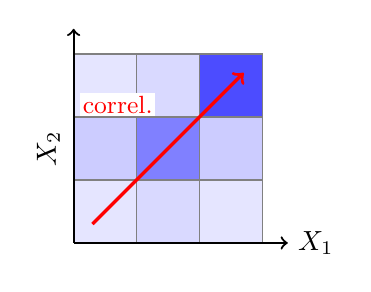
\begin{tikzpicture}[scale=0.8]
      % Empirical joint (correlated)
      \fill[blue!10] (0,0) rectangle (1,1);
      \fill[blue!50] (1,1) rectangle (2,2);
      \fill[blue!70] (2,2) rectangle (3,3);
      \fill[blue!20] (0,1) rectangle (1,2);
      \fill[blue!15] (1,0) rectangle (2,1);
      \fill[blue!10] (2,0) rectangle (3,1);
      \fill[blue!10] (0,2) rectangle (1,3);
      \fill[blue!15] (1,2) rectangle (2,3);
      \fill[blue!20] (2,1) rectangle (3,2);
      \draw[step=1,gray,thin] (0,0) grid (3,3);
      \draw[->,thick] (0,0) -- (3.4,0) node[right] {$X_1$};
      \draw[->,thick] (0,0) -- (0,3.4);
      \node[rotate=90] at (-0.4,1.5) {$X_2$};
      % Diagonal arrow
      \draw[->,red,very thick] (0.3,0.3) -- (2.7,2.7);
      \node[red,fill=white,inner sep=1pt,font=\small] at (0.7,2.2) {correl.};
    \end{tikzpicture}
    
    \vspace{0.3em}
    {\small Mass concentrated on diagonal}
  \end{column}
  
  \begin{column}{0.48\textwidth}
    \centering
    \textbf{$\windep$ (independence)}\\[0.4em]
    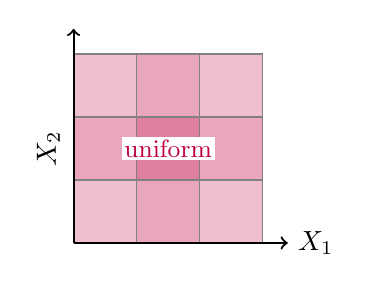
\begin{tikzpicture}[scale=0.8]
      % Independence assumed
      \fill[purple!25] (0,0) rectangle (1,1);
      \fill[purple!35] (1,0) rectangle (2,1);
      \fill[purple!25] (2,0) rectangle (3,1);
      \fill[purple!35] (0,1) rectangle (1,2);
      \fill[purple!50] (1,1) rectangle (2,2);
      \fill[purple!35] (2,1) rectangle (3,2);
      \fill[purple!25] (0,2) rectangle (1,3);
      \fill[purple!35] (1,2) rectangle (2,3);
      \fill[purple!25] (2,2) rectangle (3,3);
      \draw[step=1,gray,thin] (0,0) grid (3,3);
      \draw[->,thick] (0,0) -- (3.4,0) node[right] {$X_1$};
      \draw[->,thick] (0,0) -- (0,3.4);
      \node[rotate=90] at (-0.4,1.5) {$X_2$};
      \node[purple,fill=white,inner sep=1pt,font=\small] at (1.5,1.5) {uniform};
    \end{tikzpicture}
    
    \vspace{0.3em}
    {\small $\windep = w(x_1) \cdot w(x_2)$}
  \end{column}
\end{columns}

\vspace{0.5em}
\begin{block}{Key difference}
\small
$\wemp$ captures where data lives (diagonal). $\windep$ spreads mass uniformly, ignoring correlation.
\end{block}
\end{frame}

% ============================================================
\begin{frame}{Laplace Smoothing: Handling Empty Bins}
\small
\begin{columns}[T]
  \begin{column}{0.55\textwidth}
    \textbf{Problem:} Some bins may have zero training samples.
    \begin{itemize}
      \item Weighted mean becomes undefined (0/0)
      \item Rare regions get ignored entirely
      \item Sensitive to sampling noise
    \end{itemize}
    
    \vspace{0.8em}
    \textbf{Solution: Laplace (add-one) smoothing}
    \[
    \wlap = \wemp + \wunif
    \]
    
    \vspace{0.3em}
    Equivalently: add a ``pseudo-count'' of 1 to each bin before computing weights.
    
    \vspace{0.8em}
    \textbf{Effect:}
    \begin{itemize}
      \item Empty bins get small but non-zero weight
      \item Popular bins still dominate
      \item Interpolates between empirical and uniform
    \end{itemize}
  \end{column}
  
  \begin{column}{0.43\textwidth}
    \centering
    \textbf{Before: Empirical only}\\[0.3em]
    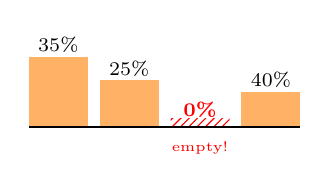
\begin{tikzpicture}[scale=0.75]
      \fill[orange!60] (0,0) rectangle (1,1.2);
      \fill[orange!60] (1.2,0) rectangle (2.2,0.8);
      \fill[red!30,pattern=north east lines,pattern color=red] (2.4,0) rectangle (3.4,0.15);
      \fill[orange!60] (3.6,0) rectangle (4.6,0.6);
      \draw[thick] (0,0) -- (4.6,0);
      \node[font=\scriptsize] at (0.5,1.4) {35\%};
      \node[font=\scriptsize] at (1.7,1.0) {25\%};
      \node[font=\scriptsize,red] at (2.9,0.3) {\textbf{0\%}};
      \node[font=\scriptsize] at (4.1,0.8) {40\%};
      \node[font=\tiny,red] at (2.9,-0.35) {empty!};
    \end{tikzpicture}
    
    \vspace{1.2em}
    \textbf{After: Laplace smoothed}\\[0.3em]
    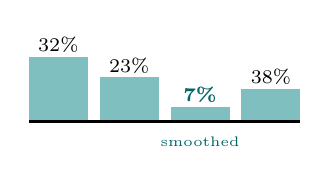
\begin{tikzpicture}[scale=0.75]
      \fill[teal!50] (0,0) rectangle (1,1.1);
      \fill[teal!50] (1.2,0) rectangle (2.2,0.75);
      \fill[teal!50] (2.4,0) rectangle (3.4,0.25);
      \fill[teal!50] (3.6,0) rectangle (4.6,0.55);
      \draw[thick] (0,0) -- (4.6,0);
      \node[font=\scriptsize] at (0.5,1.3) {32\%};
      \node[font=\scriptsize] at (1.7,0.95) {23\%};
      \node[font=\scriptsize,teal!80!black] at (2.9,0.45) {\textbf{7\%}};
      \node[font=\scriptsize] at (4.1,0.75) {38\%};
      \node[font=\tiny,teal!80!black] at (2.9,-0.35) {smoothed};
    \end{tikzpicture}
    
    \vspace{1em}
    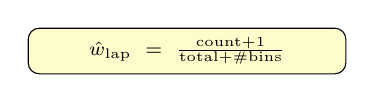
\begin{tikzpicture}
      \node[draw,rounded corners,fill=yellow!20,font=\scriptsize,text width=3.8cm,align=center] {
        $\wlap = \frac{\text{count} + 1}{\text{total} + \text{\#bins}}$
      };
    \end{tikzpicture}
  \end{column}
\end{columns}

\vspace{0.3em}
\TakeawayBox{Laplace smoothing prevents division-by-zero and ensures all bins contribute to the ``slice mean zero'' constraint.}
\end{frame}

	% ============================================================
	
	% ============================================================
		\section{Experiment 1: German Credit}

% ============================================================
\begin{frame}{Our additions: two experiments}
\small
\begin{block}{Experiment 1 (Real data): German Credit}
\begin{itemize}\itemsep0.1em
  \item Fit depth-2 XGBoost (piecewise-constant $\Rightarrow$ tensorized effects)
  \item Purify same tensors under $\wemp,\;\wunif,$ and $\windep$
  \item Hypothesis: ignoring dependence in $w$ reallocates mass between mains and interactions.
\end{itemize}
\end{block}

\begin{block}{Experiment 2 (Synthetic): stress-test under strong dependence}
\begin{itemize}\itemsep0.1em
  \item Control dependence with $\rhoVal\in\{0,0.3,0.6,0.9,0.97\}$
  \item Compare purification under $\wemp$ vs misspecified $w$ ($\wunif$/$\windep$/$\wperm$)
  \item Track divergence metrics and visualize surfaces
  \item Hypothesis: sensitivity to misspecified $w$ increases with $\rhoVal$.
\end{itemize}
\end{block}
\end{frame}

% ============================================================
\begin{frame}{Experiment 1: German Credit (setup)}
\small
\begin{block}{ML hygiene}
\begin{itemize}\itemsep0.1em
  \item Target: \texttt{Credit amount} (regression). Split: 75/25 train/test.
  \item Preprocessing: fill missing with \texttt{unknown}, one-hot encode categoricals.
\end{itemize}
\end{block}

\begin{block}{Model + purification}
\begin{itemize}\itemsep0.1em
  \item Model: depth-2 XGBoost (n\_estimators=120, lr=0.1).
  \item Binning: thresholds from tree splits (fixed across $w$).
  \item Purification: compare $\wemp$, $\wunif$, and $\windep$.
\end{itemize}
\end{block}

\begin{block}{What to look for}
Does the qualitative explanation (sign, monotonicity, quadrant pattern) change when dependence is ignored in $w$?
\end{block}
\end{frame}

% ============================================================
\begin{frame}{German Credit: Summary Statistics}
\small
\begin{block}{Prediction invariance confirmed}
RMSE = 2043.3 across all weight modes ($\wemp$, $\wunif$, $\windep$) --- predictions are \textbf{identical}.
\end{block}

\begin{columns}[T]
\begin{column}{0.48\textwidth}
\begin{block}{Top main effects (by variance)}
\scriptsize
\begin{tabular}{lr}
\textbf{Feature} & \textbf{Var} \\ \hline
Duration & 2,906,619 \\
Job\_3 & 247,365 \\
Purpose\_vacation & 93,542 \\
Age & 79,656 \\
Purpose\_radio/TV & 43,529 \\
\end{tabular}
\end{block}
\end{column}
\begin{column}{0.48\textwidth}
\begin{block}{Top interactions (by variance)}
\scriptsize
\begin{tabular}{lr}
\textbf{Pair} & \textbf{Var} \\ \hline
Duration $\times$ Purpose\_vac & 29,522 \\
Age $\times$ Duration & 17,139 \\
Duration $\times$ Job\_3 & 7,498 \\
Saving\_mod $\times$ Purp\_edu & 5,888 \\
\end{tabular}
\end{block}
\end{column}
\end{columns}

\TakeawayBox{\textbf{Duration} dominates mains; its effect depends on loan purpose (interaction). Different $w$ reallocates variance but predictions stay identical.}
\end{frame}

% ============================================================
\begin{frame}{German Credit: main effects (top features)}
\centering
\begin{columns}[T,onlytextwidth]
  \begin{column}{0.49\textwidth}
    \centering
    \includegraphics[width=\linewidth,height=0.72\textheight,keepaspectratio,viewport=0 475.2 612 950.4,clip]{\resultsdir german_credit_top_mains.pdf}
  \end{column}
  \begin{column}{0.49\textwidth}
    \centering
    \includegraphics[width=\linewidth,height=0.72\textheight,keepaspectratio,viewport=0 0 612 475.2,clip]{\resultsdir german_credit_top_mains.pdf}
  \end{column}
\end{columns}
\TakeawayBox{Same model and binning; differences across $w$ are reallocations between mains and interactions.}
\end{frame}

% ============================================================
\begin{frame}{German Credit: top interaction heatmap}
\centering
\includegraphics[width=0.98\linewidth,height=0.78\textheight,keepaspectratio]{\resultsdir german_credit_top_interaction_heatmap.pdf}
\TakeawayBox{Interaction residual after purification. If $\windep$ changes the qualitative pattern relative to $\wemp$, the interaction story is sensitive to ignoring dependence.}
\end{frame}


% ============================================================
	\section{Experiment 2: Stress-test under strong dependence}

\begin{frame}{Experiment 2: core question (weighting distribution $w$)}
\small
\begin{block}{Question}
Under strong feature dependence, how much do purified mains/interactions change when we purify using:
\begin{itemize}
  \item the \textbf{correct joint} (empirical $\wemp \approx p(x)$) vs
  \item a \textbf{misspecified} weighting (uniform or independence-assumed)?
\end{itemize}
\end{block}

\begin{itemize}
  \item Same learned piecewise-constant model $\Rightarrow$ same tensors.
  \item Only $w$ changes.
\end{itemize}
\end{frame}

% ============================================================
\begin{frame}{Stress-test: data generation}
\small
\begin{block}{Linear-Gaussian dependence}
\[
X_1 \sim \mathcal{N}(0,1),\quad \varepsilon \sim \mathcal{N}(0,1)\ \text{independent}
\]
\[
X_2 = \rhoVal X_1 + \sqrt{1-\rhoVal^2}\,\varepsilon,
\quad \rhoVal \in \{0.0,0.3,0.6,0.9,0.97\}
\]
\end{block}

\begin{block}{Ground-truth functions}
\begin{itemize}
  \item (F1) $F(X_1,X_2)=\beta_1X_1+\beta_2X_2+\gamma(X_1X_2)$
  \item (F2) $F(X_1,X_2)=\gamma\,\mathrm{sign}(X_1)\mathrm{sign}(X_2)+\beta_1X_1+\beta_2X_2$
\end{itemize}
\end{block}
\end{frame}

% ============================================================
\begin{frame}{Evaluation Metrics: Visual Guide}
\begin{columns}[T]
  \begin{column}{0.48\textwidth}
    \centering
    \textbf{Weighted $L_2$ Distance}\\[0.5em]
    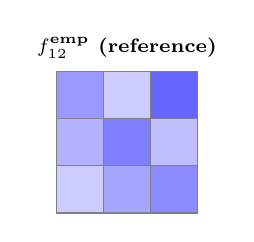
\begin{tikzpicture}[scale=0.6]
      % Reference surface
      \node[font=\scriptsize\bfseries] at (1.5,3.5) {$f_{12}^{\text{emp}}$ (reference)};
      \fill[blue!40] (0,2) rectangle (1,3);
      \fill[blue!20] (1,2) rectangle (2,3);
      \fill[blue!60] (2,2) rectangle (3,3);
      \fill[blue!30] (0,1) rectangle (1,2);
      \fill[blue!50] (1,1) rectangle (2,2);
      \fill[blue!25] (2,1) rectangle (3,2);
      \fill[blue!20] (0,0) rectangle (1,1);
      \fill[blue!35] (1,0) rectangle (2,1);
      \fill[blue!45] (2,0) rectangle (3,1);
      \draw[step=1,gray] (0,0) grid (3,3);
    \end{tikzpicture}
    \hspace{0.2em}
    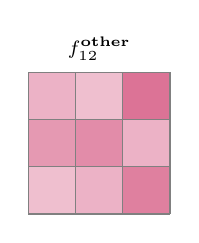
\begin{tikzpicture}[scale=0.6]
      % Comparison surface
      \node[font=\scriptsize\bfseries] at (1.5,3.5) {$f_{12}^{\text{other}}$};
      \fill[purple!30] (0,2) rectangle (1,3);
      \fill[purple!25] (1,2) rectangle (2,3);
      \fill[purple!55] (2,2) rectangle (3,3);
      \fill[purple!40] (0,1) rectangle (1,2);
      \fill[purple!45] (1,1) rectangle (2,2);
      \fill[purple!30] (2,1) rectangle (3,2);
      \fill[purple!25] (0,0) rectangle (1,1);
      \fill[purple!30] (1,0) rectangle (2,1);
      \fill[purple!50] (2,0) rectangle (3,1);
      \draw[step=1,gray] (0,0) grid (3,3);
    \end{tikzpicture}
    
    \vspace{0.3em}
    \[
    d_{L_2} = \sqrt{\sum_{i,j} w_{ij} \left(f^{\text{emp}}_{ij} - f^{\text{other}}_{ij}\right)^2}
    \]
    {\scriptsize Measures overall surface difference}
  \end{column}
  
  \begin{column}{0.48\textwidth}
    \centering
    \textbf{Sign Flip Rate}\\[0.5em]
    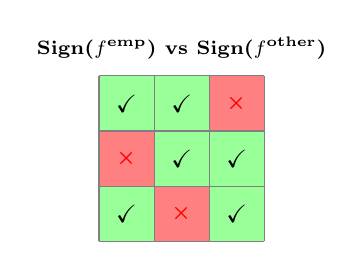
\begin{tikzpicture}[scale=0.7]
      % Sign comparison
      \node[font=\scriptsize\bfseries] at (1.5,3.5) {Sign($f^{\text{emp}}$) vs Sign($f^{\text{other}}$)};
      \fill[green!40] (0,2) rectangle (1,3);
      \fill[green!40] (1,2) rectangle (2,3);
      \fill[red!50] (2,2) rectangle (3,3);
      \fill[red!50] (0,1) rectangle (1,2);
      \fill[green!40] (1,1) rectangle (2,2);
      \fill[green!40] (2,1) rectangle (3,2);
      \fill[green!40] (0,0) rectangle (1,1);
      \fill[red!50] (1,0) rectangle (2,1);
      \fill[green!40] (2,0) rectangle (3,1);
      \draw[step=1,gray] (0,0) grid (3,3);
      \node[font=\small] at (0.5,2.5) {\checkmark};
      \node[font=\small] at (1.5,2.5) {\checkmark};
      \node[font=\small,red] at (2.5,2.5) {\texttimes};
      \node[font=\small,red] at (0.5,1.5) {\texttimes};
      \node[font=\small] at (1.5,1.5) {\checkmark};
      \node[font=\small] at (2.5,1.5) {\checkmark};
      \node[font=\small] at (0.5,0.5) {\checkmark};
      \node[font=\small,red] at (1.5,0.5) {\texttimes};
      \node[font=\small] at (2.5,0.5) {\checkmark};
    \end{tikzpicture}
    
    \vspace{0.3em}
    \[
    \text{flip rate} = \frac{\#\{\text{sign differs}\}}{\#\{\text{bins}\}} = \frac{3}{9}
    \]
    {\scriptsize Measures qualitative disagreement}
  \end{column}
\end{columns}

\vspace{0.6em}
\TakeawayBox{$L_2$ captures magnitude differences; sign flips capture qualitative interpretation changes (e.g., ``positive effect'' $\to$ ``negative effect'').}
\end{frame}

% ============================================================
\begin{frame}{Stress-test: weighting comparison + metrics}
\small
We purify the same tensors under:
\[
w \in \{\wemp,\; \wunif,\; \windep,\; \wperm\}.
\]

\vspace{0.4em}
\begin{block}{Metrics vs $\rhoVal$}
\begin{itemize}
  \item Weighted $L_2$ distance between purified interaction surfaces (reference measure: $\wemp$)
  \item Sign flip rate vs $\wemp$ (fraction of bins with sign changes)
  \item Interaction variance share: $\Varw(f_{12})/\Varw(F)$
\end{itemize}
\end{block}
\end{frame}

% ============================================================
\begin{frame}{Weight Modes Explained}
\small
\begin{tabular}{@{}lp{7.5cm}@{}}
\toprule
\textbf{Mode} & \textbf{Definition} \\
\midrule
$\wemp$ (empirical) & Observed joint distribution $\hat{p}(x_1,x_2)$ from training data. Captures dependence. \\[4pt]
$\wunif$ (uniform) & Equal weight $\frac{1}{|\Omega_1|\cdot|\Omega_2|}$ for all bin pairs. Ignores data distribution. \\[4pt]
$\windep$ (indep) & Product of marginals: $\hat{p}(x_1)\cdot\hat{p}(x_2)$. Assumes independence analytically. \\[4pt]
$\wperm$ (perm\_joint) & Shuffle columns to break dependence, then compute empirical joint. Independence via resampling. \\
\bottomrule
\end{tabular}

\vspace{0.6em}
\textbf{Key point:} Under strong feature correlation, these weight choices lead to \textbf{different purified effects}.
\end{frame}

	% ============================================================
		\begin{frame}{Stress-test (F1): $L_2$ distance vs $\rhoVal$}
		\centering
		\includegraphics[width=0.98\linewidth,height=0.72\textheight,keepaspectratio]{\resultsdir stress_dependence_l2_interaction_F1.pdf}
		\TakeawayBox{Distance from the $\wemp$-purified interaction increases with dependence; misspecified $w$ yields divergent explanations.}
		\end{frame}
	
	% ============================================================
		\begin{frame}{Stress-test (F1): sign flip rate vs $\rhoVal$}
		\centering
		\includegraphics[width=0.98\linewidth,height=0.72\textheight,keepaspectratio]{\resultsdir stress_dependence_signflip_interaction_F1.pdf}
		\TakeawayBox{As dependence grows, qualitative interaction conclusions (sign) become sensitive to the choice of $w$.}
		\end{frame}
	
	% ============================================================
		\begin{frame}{Stress-test (F1): interaction variance share vs $\rhoVal$}
		\centering
		\includegraphics[width=0.98\linewidth,height=0.72\textheight,keepaspectratio]{\resultsdir stress_dependence_interaction_share_F1.pdf}
		\TakeawayBox{Variance attribution to the interaction changes with $w$; under dependence, misspecifying $w$ reshuffles main vs interaction credit.}
		\end{frame}
	
	% ============================================================
		\begin{frame}{Stress-test (F2): $L_2$ distance vs $\rhoVal$}
		\centering
		\includegraphics[width=0.98\linewidth,height=0.72\textheight,keepaspectratio]{\resultsdir stress_dependence_l2_interaction_F2.pdf}
		\TakeawayBox{Distance from the $\wemp$-purified interaction increases with dependence; misspecified $w$ yields divergent explanations.}
		\end{frame}
	
	% ============================================================
		\begin{frame}{Stress-test (F2): sign flip rate vs $\rhoVal$}
		\centering
		\includegraphics[width=0.98\linewidth,height=0.72\textheight,keepaspectratio]{\resultsdir stress_dependence_signflip_interaction_F2.pdf}
		\TakeawayBox{As dependence grows, qualitative interaction conclusions (sign) become sensitive to the choice of $w$.}
		\end{frame}
	
	% ============================================================
		\begin{frame}{Stress-test (F2): interaction variance share vs $\rhoVal$}
		\centering
		\includegraphics[width=0.98\linewidth,height=0.72\textheight,keepaspectratio]{\resultsdir stress_dependence_interaction_share_F2.pdf}
		\TakeawayBox{Variance attribution to the interaction changes with $w$; under dependence, misspecifying $w$ reshuffles main vs interaction credit.}
		\end{frame}

% ============================================================
\begin{frame}{Stress-test: Summary --- $L_2$ Distance \& Sign Flips}
\small
\begin{block}{$L_2$ distance (interaction surface vs $\wemp$ reference)}
\centering
\begin{tabular}{l|cc|cc}
 & \multicolumn{2}{c|}{\textbf{F1 (multiplicative)}} & \multicolumn{2}{c}{\textbf{F2 (XOR-like)}} \\
\textbf{Mode} & $\rho{=}0$ & $\rho{=}0.97$ & $\rho{=}0$ & $\rho{=}0.97$ \\ \hline
uniform & 0.31 & 0.27 & 0.14 & \textbf{0.88} \\
indep & 0.17 & 0.32 & 0.14 & \textbf{0.90} \\
perm\_joint & 0.22 & 0.32 & 0.20 & \textbf{0.87} \\
\end{tabular}
\end{block}

\begin{block}{Sign flip rate at $\rho=0.97$}
\centering
\begin{tabular}{l|cc}
\textbf{Mode} & \textbf{F1} & \textbf{F2} \\ \hline
uniform & 29\% & 17\% \\
indep & 28\% & 19\% \\
\end{tabular}
\end{block}

\TakeawayBox{At high $\rho$, F2 shows $L_2 \approx 0.9$ (surface almost unrecognizable). 20--30\% of bins flip sign!}
\end{frame}

% ============================================================
\begin{frame}{Stress-test: Summary --- Variance Attribution}
\small
\begin{block}{Interaction variance share: $\Varw(f_{12})/\Varw(F)$}
\centering
\begin{tabular}{l|cc|cc}
 & \multicolumn{2}{c|}{\textbf{F1}} & \multicolumn{2}{c}{\textbf{F2}} \\
\textbf{Mode} & $\rho{=}0$ & $\rho{=}0.97$ & $\rho{=}0$ & $\rho{=}0.97$ \\ \hline
$\wemp$ & 29\% & \textbf{0.002\%} & 80\% & \textbf{5.6\%} \\
uniform & 36\% & 5.6\% & 78\% & 59\% \\
indep & 33\% & 1.4\% & 84\% & \textbf{73\%} \\
\end{tabular}
\end{block}

\vspace{0.3em}
\begin{alertblock}{Key insight}
For F1 at $\rho{=}0.97$: $\wemp$ shows \textbf{0\% interaction} (absorbed into mains).\\
But $\windep$ reports 1.4\%, $\wunif$ reports 5.6\% --- \textbf{qualitatively different stories!}
\end{alertblock}

\TakeawayBox{Variance attribution shifts dramatically with $w$; misspecifying $w$ yields misleading importance rankings.}
\end{frame}
	
	% ============================================================
		\begin{frame}{Stress-test (F1): interaction heatmaps at $\rhoVal=0.97$}
		\centering
		\includegraphics[width=0.98\linewidth,height=0.74\textheight,keepaspectratio]{\resultsdir stress_dependence_heatmaps_F1_rho0.97.pdf}
		\TakeawayBox{At strong dependence ($\rhoVal=0.97$), the interaction surface can change noticeably across $w$; $\wemp$ emphasizes where samples occur.}
		\end{frame}
	
	% ============================================================
		\begin{frame}{Stress-test (F2): interaction heatmaps at $\rhoVal=0.97$}
		\centering
		\includegraphics[width=0.98\linewidth,height=0.74\textheight,keepaspectratio]{\resultsdir stress_dependence_heatmaps_F2_rho0.97.pdf}
		\TakeawayBox{At strong dependence ($\rhoVal=0.97$), the interaction story depends on $w$; misspecification can change qualitative patterns.}
		\end{frame}

% ============================================================
	\begin{frame}{Stress-test: main effect curves at $\rhoVal=0.97$ (F1 example)}
	\centering
	\includegraphics[width=0.98\linewidth,height=0.78\textheight,keepaspectratio]{\resultsdir stress_dependence_mains_F1_rho0.97.pdf}
	\TakeawayBox{Main-effect curves can shift across $w$ even when the model is fixed; changes are compensating reallocations with interactions (prediction stays the same).}
	\end{frame}

% ============================================================
\begin{frame}{Conclusions}
\begin{block}{Theoretical contribution (paper)}
\begin{itemize}\itemsep0.2em
  \item Interactions are \textbf{not identifiable} without constraints; fANOVA yields a canonical decomposition under $w$.
  \item Purification: exact post-hoc mass-moving recovers fANOVA for piecewise-constant models.
\end{itemize}
\end{block}

\begin{block}{Our experimental findings}
\begin{itemize}\itemsep0.2em
  \item \textbf{Predictions are invariant} to weight choice (confirmed: identical RMSE across $w$).
  \item \textbf{Interpretations are NOT invariant}: under strong dependence ($\rho{=}0.97$):
  \begin{itemize}
    \item Variance attribution shifts dramatically (0\% vs 73\% interaction share)
    \item 20--30\% of bins flip sign
    \item $L_2$ distance up to 0.9 (interaction surface almost unrecognizable)
  \end{itemize}
\end{itemize}
\end{block}

\TakeawayBox{Always report which $w$ you used. Treat $\wemp$ vs $\windep$ as a \textbf{sensitivity analysis} when feature dependence is plausible.}
\end{frame}

% ============================================================
\begin{frame}{References \& Resources}
\small
\begin{block}{Original Paper}
Lengerich, B., Tan, S., Chang, C.-H., Hooker, G., \& Caruana, R. (2020).\\[0.3em]
\textit{Purifying Interaction Effects with the Functional ANOVA: An Efficient Algorithm for Recovering Identifiable Additive Models}.\\[0.3em]
AISTATS 2020, PMLR 108:2402--2412.\\[0.5em]
\url{https://proceedings.mlr.press/v108/lengerich20a.html}
\end{block}

\vspace{0.1em}
\begin{block}{Code \& Related Projects}
\begin{itemize}
  \item Original paper implementation: \url{https://github.com/blengerich/gam_purification}
  \item InterpretML (Microsoft): \url{https://github.com/interpretml/interpret}
\end{itemize}
\end{block}

\vspace{0.1em}
\begin{block}{Dataset}
German Credit Data --- UCI Machine Learning Repository\\[0.3em]
\url{https://archive.ics.uci.edu/ml/datasets/statlog+(german+credit+data)}
\end{block}
\end{frame}

% ============================================================
\begin{frame}{AI Usage Disclosure}
\begin{block}{AI Tools Used}
The following AI tools were used to support development of this project:
\begin{itemize}
  \item \textbf{NotebookLM} (Google) --- understanding the paper
  \item \textbf{ChatGPT 5.2 Pro} (OpenAI) --- code generation, debugging, and slide drafting
  \item \textbf{Claude Opus / Sonnet 4.5} (Anthropic) --- code review, documentation, and slide refinement
\end{itemize}
\end{block}

\vspace{1em}
{\centering All AI-generated content was reviewed, validated, and edited by the author.\par}
\end{frame}

\end{document}
